%%%% Header %%%%%%%%%%%%%%%%%%%%%%%%%%%%%%%%%%%%%%%%%%%%%%%%%%%%%%%%%%%%%%%%%%%

\documentclass[
  10pt
]{scrartcl}

\usepackage{jonas}

\bibliography{/home/jon/lucile/share/jowncloud/sci/refs/refs.bib}
\hyphenation{}

%%%% Meta data %%%%%%%%%%%%%%%%%%%%%%%%%%%%%%%%%%%%%%%%%%%%%%%%%%%%%%%%%%%%%%%%

\usepackage[
  pdfauthor   ={Jonas Schöley},
  pdftitle    ={},
  pdfsubject  ={},
  pdfkeywords ={},
  pdfproducer =Latex,
  pdfcreator  =pdflatex
]{hyperref}

\title{Life Expectancy at Birth versus Lifespan Equality}
\author{Jonas Schöley}

%%%% Titlepage %%%%%%%%%%%%%%%%%%%%%%%%%%%%%%%%%%%%%%%%%%%%%%%%%%%%%%%%%%%%%%%%

\begin{document}

\maketitle

%\begin{abstract}
%\end{abstract}

%%%% Text %%%%%%%%%%%%%%%%%%%%%%%%%%%%%%%%%%%%%%%%%%%%%%%%%%%%%%%%%%%%%%%%%%%%%

\begin{table}[ht!]
\tabformat
  \begin{tabular}{m{0.3\textwidth}m{0.5\textwidth}}
  \toprule
  Average $l_x$ & $$\overline{l_x} = \frac{\int_0^\omega l_x^2 \,dx} {e_0}$$ \\
  \midrule
  Inverse Gini Coefficient of Average $l_x$ & $$G\overline{l_x} = \left(1 - \overline{l_x}\right)^{-1}$$ \\
  \midrule
  Logit of Average $l_x$ & $$\text{logit}~\overline{l_x} = \frac{\overline{l_x}} {1 - \overline{l_x}}$$ \\
  \midrule
  Inverse Keyfitz' Entropy & $$H^{-1} = -\left(\frac{\int_0^\omega l_x \times \log l_x\,dx} {e_0}\right)^{-1}$$ \\
  \midrule
  Outer Rectangularization (ORR) & $$ORR = \frac{e_0} {\omega}$$\\
  \midrule
  Maximum Inner Rectangle of $l_x$ (MIRA) & $$A = \max_{x \in \mathbb{N}}(l_x \cdot x)$$ \\
  \midrule
  Inner Rectangularization (IRR) & $$IRR = \frac{\max_{x \in \mathbb{N}}(l_x \cdot x)} {\omega}$$ \\
  \midrule
  Inverse Interquartile Range of $l_x$ & $$IQR^{-1}~l_x = \left(\arg_x (l_x = 0.25) - \arg_x (l_x = 0.75)\right)^{-1}$$ \\
  \bottomrule
  \end{tabular}
  \caption{Measures of lifespan equality.}
\end{table}

\begin{figure}[ht!]
  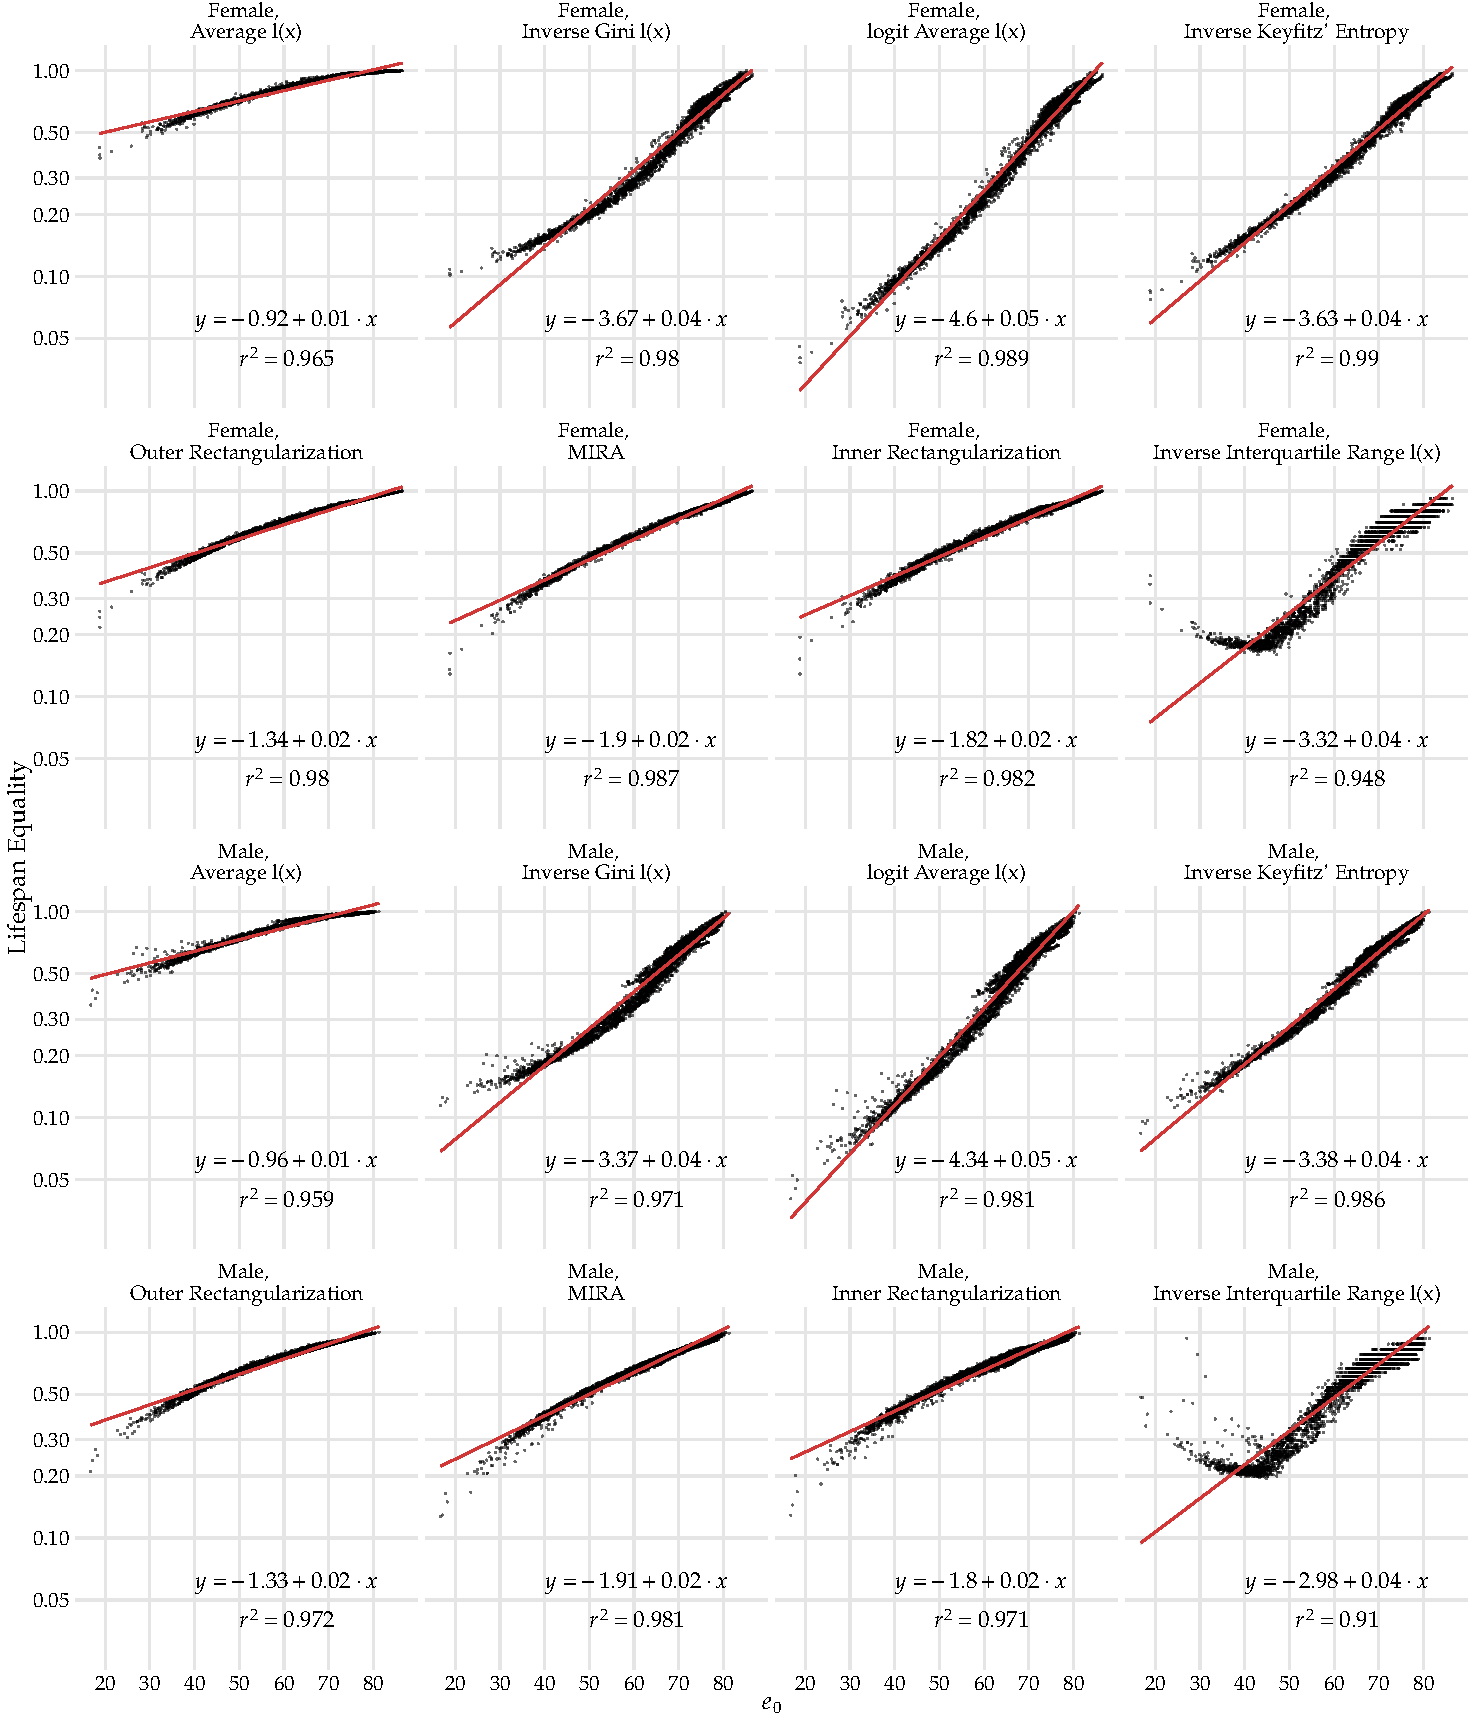
\includegraphics[width = \linewidth]{../out/plot_e0_vs_lx_equality.pdf}
  \caption{Different measures of lifespan disparity plotted versus life expectancy at birth. \emph{Data source: HMD, male and female period lifetables.}}
\end{figure}

\begin{figure}[ht!]
  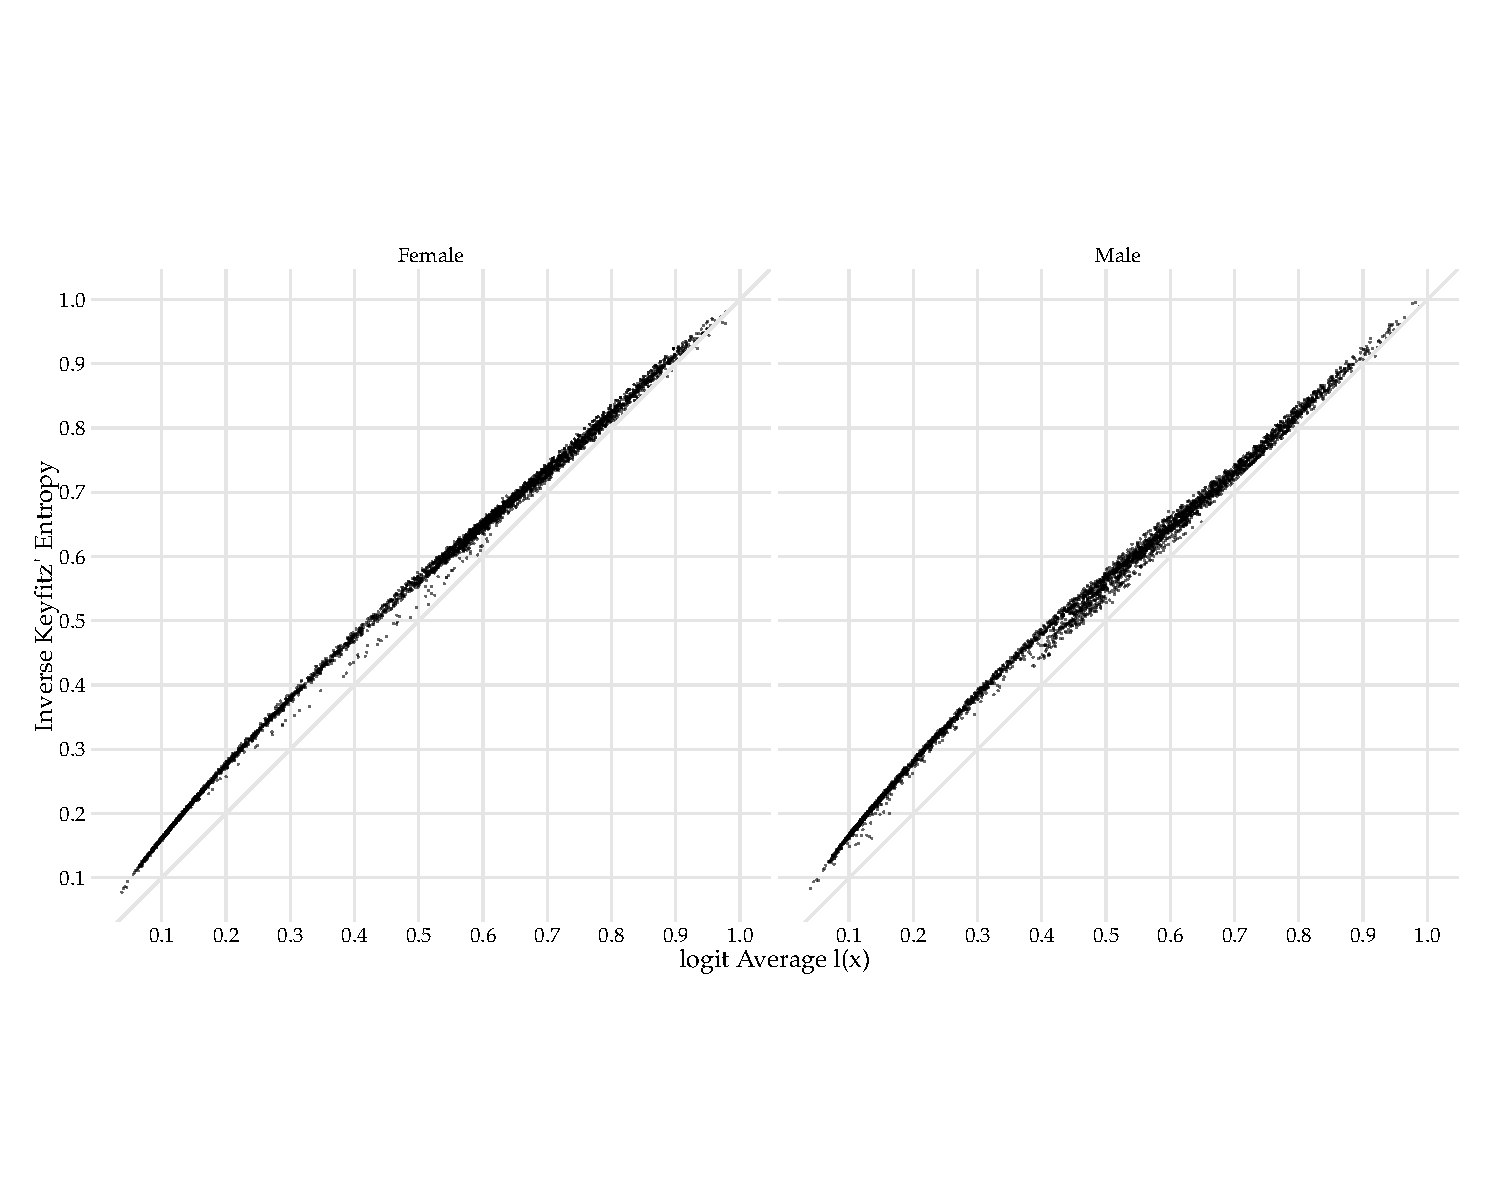
\includegraphics[width = \linewidth]{../out/plot_logitavglx_vs_keyfentr.pdf}
  \caption{Logit of average $l_x$ against Keyfitz' entropy. \emph{Data source: HMD, male and female period lifetables.}}
\end{figure}

\begin{figure}[ht!]
  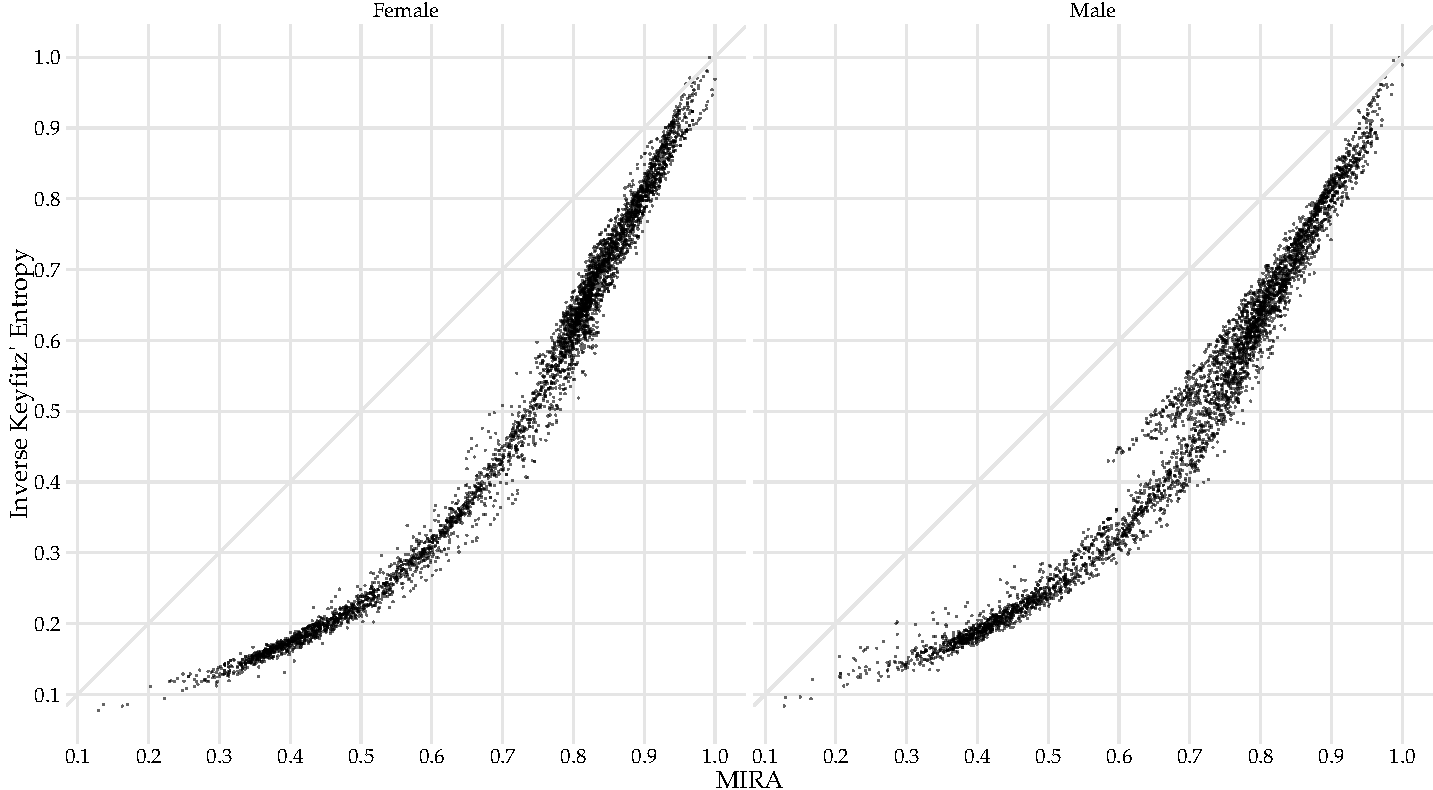
\includegraphics[width = \linewidth]{../out/plot_mira_vs_keyfentr.pdf}
  \caption{Maximum inner rectangle of $l_x$ against Keyfitz' entropy. \emph{Data source: HMD, male and female period lifetables.}}
\end{figure}

\clearpage

%%%% Bibliography %%%%%%%%%%%%%%%%%%%%%%%%%%%%%%%%%%%%%%%%%%%%%%%%%%%%%%%%%%%%%

\sloppy
\printbibliography

%\clearpage

%%%% Appendix %%%%%%%%%%%%%%%%%%%%%%%%%%%%%%%%%%%%%%%%%%%%%%%%%%%%%%%%%%%%%%%%%

% appendix figures follow A1, A2, B1... scheme
%\renewcommand\thefigure{\thesection.\arabic{figure}}
%\setcounter{figure}{0}

%\begin{appendix}
%\end{appendix}

\end{document}